\begin{frame}{LAVORO DI TESI}
    Lo studio della tesi si è concentrato sulla ricerca e sull'implementazione 
    di varie tecniche di compressione e, allo stesso tempo, di ottimizzazione, 
    in grado di offrire supporto allo sviluppo di un nuovo modello di guida autonoma efficiente e ad alta velocità di inferenza.\\
    \vspace{0.3cm}
    Quest'ultimo, deriva dallo studio di due modelli già noti allo stato dell'arte:
    \begin{minipage}{\linewidth}
        \centering
        \begin{minipage}{0.45\linewidth}
            \begin{enumerate}
                \item {\bfseries{\emph{MobileNet-V1}}}\footnotemark[1]: specializzato nel task di \emph{Image classification};
                \item {\bfseries{\emph{Single-Shot-Detector (SSD)}}}\footnotemark[2]: specializzato nel task di \emph{Object Detection}.
            \end{enumerate}
        \end{minipage}
        \begin{minipage}{0.45\linewidth}
            \begin{figure}
                \centering
                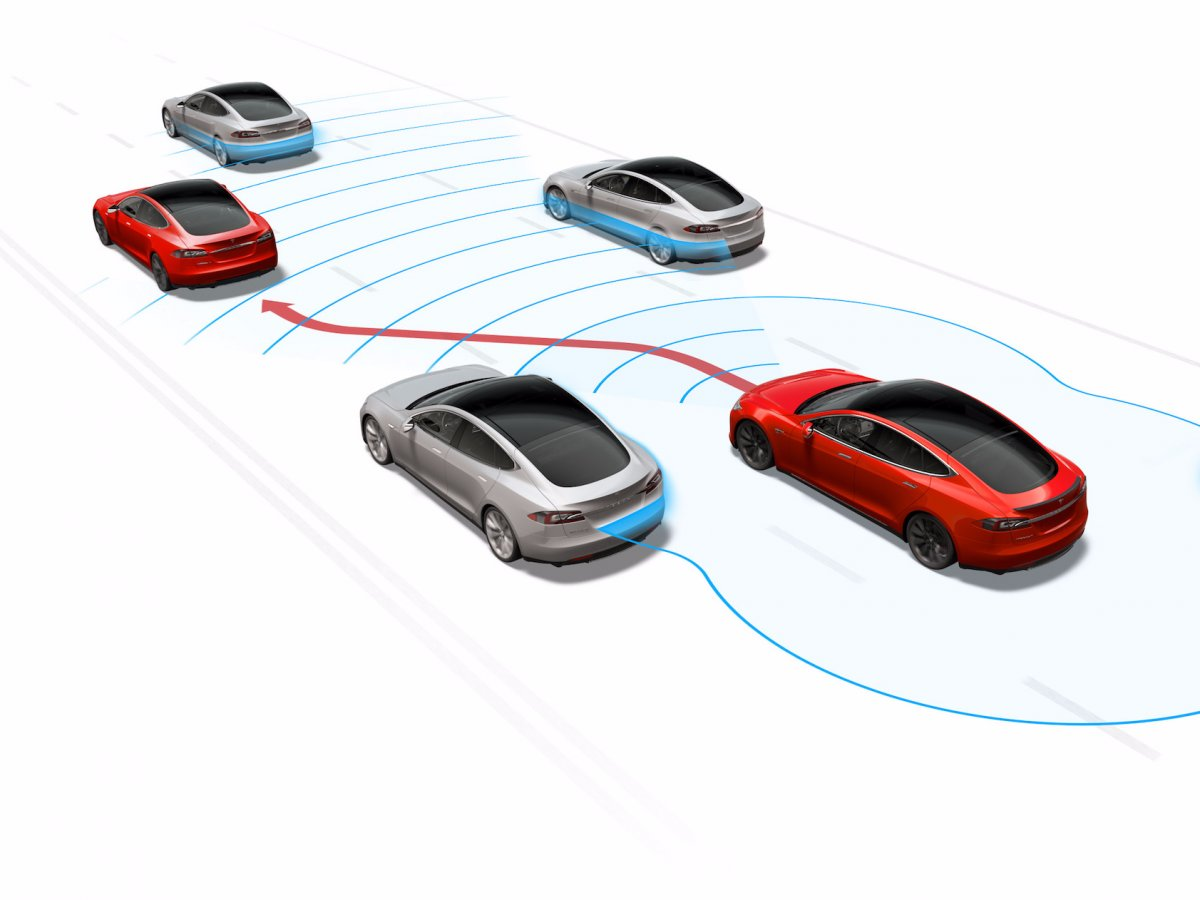
\includegraphics[width = \linewidth]{tesla_autopilot.png}
                \centering
            \end{figure}
        \end{minipage}
    \end{minipage}
    \footnotetext[1]{\emph{Andrew G. Howard et al., "MobileNets: Efficient Convolutional Neural Networks for Mobile Vision Applications", 2017.}}
    \footnotetext[2]{\emph{Liu et al., "SSD: Single Shot MultiBox Detector", 2016.}}
\end{frame}